\section{Requirements and System Model}\label{sec:requirements}
Big data is highly dependent on cloud-edge computing, which makes extensive use of multitenancy.
Multitenancy permits sharing one instance of infrastructures, platforms or applications by multiple tenants to optimize costs.
This leads to common scenarios where a service provider offers subscription-based analytics capabilities in the cloud,
or a single data lake is accessed by multiple customers.
Thus, it is a common situation to have a big data pipeline where data and services belong to various organizations,
posing a serious risk of potential privacy and security violation.
In the following of this section,
we present our system model (Section \ref{sec:systemmodel}),
the requirements driving our work (Section \ref{sec:accesscontrol_req}),
and our reference scenario (Section \ref{sec:reference}).
\AG{
  The fundamental concept underlying our methodology is to enhance the prevailing paradigm for big data pipelines through the creation of a Data Governance framework tailored to contemporary data-driven pipelines.
  The primary objective of this framework is to facilitate the assembly of data processing services, with a central focus on the selection of these services to optimize data quality, all while upholding privacy standards.
}

\subsection{System Model}\label{sec:systemmodel}
\AG{
  In our context, a \user aims to execute a data pipeline to perform some analysis or transformation procedures on some data.
  The input data are considered alredey cleaned,
  Policies governing the data are established, which can originate from the \user, third-party entities, or regulatory frameworks.
  For instance, a policy may restrict the execution of processing operations to a specific geographic region.
  The \user is provided with a set of empty pipeline templates. Each template represents a blank pipeline with the necessary steps but without the specific services.
  The user is given the opportunity to choose, for each step of the template, from a collection of candidate services that are functionally equivalent and comply with the specified policies.
  By selecting the most suitable service template from a range of available options,
  the \user ensures an alignment between the service composition and their distinctive demands.
  These services are subsequently ranked based on their ability to retain the maximum amount of data while maintaining an equivalent level of privacy.
  Underlying our investigation is the assumption that a greater quantity of preserved data corresponds to enhanced data quality.
}

Our reference scenario is a service-based environment where services are composed according to a pipeline template.

It includes the following parties:
i) User: the entity that wants to perform some analytics on the data
ii) Pipeline: a sequence of connected services that process and move data from one point to another in a structured and automated manner.
iii) Service: a software that performs a specific task, a service is characterized by two function: the service function and the policy function.
iv) Service composition: the process of combining two or more services to create a new service
v) Policy: a structured set of guidelines, rules, and procedures that define how the service must safeguards its data to maintain confidentiality
% \begin{itemize}
%   \item User owns some data and wants to perform some analytics on it
%   \item Choose a pipeline template and a wanted level of privacy
%   \item The template has lambda, signed
%   \item Policy is a set of rules
%   \item Match the policy with the lambda
%   \item Compares services that match the policy ranking them based on quality
%   \item Choose the best service
%   \item The composite service is executed
% \end{itemize}

\AG{
  The rise in data production has led the scientific community to split into two main areas of focus.
  On one side, researchers are working on ways to make the most of the valuable data we have.
  On the other side, there's a growing need to keep data safe and private.
  These two directions are happening at the same time, but there are not many solutions that find a good balance between them.
  So, the solution we propose aims to create a framework that can strike a balance between privacy and data quality.
  We want to get as much quality from the data as possible while still protecting privacy.
  Our system model aims to achieve an optimal service composition to ensure privacy and data quality.
  Within this context, we contemplate an interconnected sequence of services, establishing a pipeline where individual nodes signify distinct services.
  Each stage within the pipeline undertakes the task of data transformation or processing, with the resulting output serving as the input for the subsequent service.
  This model encapsulates what we refer to as a template, visually presented in Figure \ref{fig:service_composition_template}.
  In order to instantiate the template, the selection of services to be executed at each step of the pipeline becomes imperative.
  At each step, there exists a set of functionally equivalent candidate services (\s{0}\dots\s{n}) that differ in terms of annotation and data transformation.
  These services are annotated with a set of requirements that encompass crucial details
  The annotations play a pivotal role in the creation of policies that determine the eligibility of a service for deployment.
  By enforcing such policies, the set of candidate services for a given step is reduced.
  The remaining services undergo evaluation based on their potential impact on the data transformation process.
  Preference is given to the service that maximizes data quality while ensuring an equal level of data privacy.
  This evaluation process aids in identifying the most suitable service for a particular step in the pipeline.
  Upon the selection of the most appropriate service for each step, the instantiation of the pipeline is deemed complete.
  Consequently, the pipeline becomes ready for execution, with the assurance that the chosen services align with the specified requirements and optimize the desired outcomes.
}
\subsection{Service Flow}
Within the framework, a service is defined as an entity that receives input data, processes it by applying a transformation function, and produces an output result. Each service essentially consists of two parts:
\begin{enumerate}
  \item The service transformation function (\Transformation{F}{\myGamma}).
  \item The policy transformation function (\Transformation{P}{\myLambda}).
\end{enumerate}
Where \myGamma and \myLambda are instrumentations of the service. That is, the service is tagged with \myLambda and \myGamma.

The execution of a service can be conceptually divided into 4 phases:
\begin{enumerate}
  \item Policy enforcement: The framework applies the service policy (\Transformation{P}{\myGamma})
        to the data. This may typically involve transforming or filtering the dataset.
  \item Data reception: The service receives input data from the user or from the service preceding it in the workflow. The received data is averaged by the framework via application of the previous step. The data that the service receives is therefore to be considered privacy ready.
  \item Service function execution: The Service applies its processing function. The function can be of 4 main types:
        \begin{itemize*}
          \item \F{Empty} The function applies no transformation or processing on the data.
          \item \F{additive} The function expands the amount of data received, for example, by integrating it with data from other sources.
          \item \F{transformation} The function transforms some records in the dataset without altering the domain.
          \item \F{domain change }  The function changes the domain of the data by applying e.g. PCA or Kmeans (will not be considered in the current work).
        \end{itemize*}
  \item Calculation of metrics $\rightarrow$ The framework calculates the quality metrics on the dataset produced downstream of the application of the function.
\end{enumerate}
Output of the result $\rightarrow$ the obtained dataset is brought to the output.


In essence, the execution of a service can be conceptualized as a multi-stage process, wherein input data is received, subjected to a defined function, quality metrics are assessed, policy is applied, further metrics are computed, and the ultimate result is readied for further application or analysis.
% We formally model a Big Data analytics pipeline as follows.

% \begin{definition}[Big Data Analytics Pipeline] \label{def:pipeline}
%   A Big Data Analytics pipeline \G(\V,\E) is a direct acyclic graph having a root \vi{r}$\in$\V, a vertex \vi{i}$\in$\V$_I$$\subseteq$\V\ for each job \job{i} invocation, two additional vertices \vi{c},\vi{m}$\in$\V$_{\otimes}$$\subset$\V\ for each alternative ($\otimes$) structure modeling the alternative execution (\emph{choice}) of operations and the retrieval (\emph{merge}) of the results,
%     respectively, and two additional vertices \vi{f},\vi{j}$\in$\V$_{\oplus}$$\subset$\V\ for each parallel ($\oplus$) structure modeling the contemporary execution (\emph{fork}) of operations and the integration (\emph{join}) of their results, respectively.
% \end{definition}

% We note that each vertex \vi{i} model a job \job{i} provided by an organization \org{i}.
% We also note that an analytics pipeline can be deployed following a centralized or a decentralized approach as discussed in detail in Section \ref{sec:architecture}.

\begin{figure}[!t]
  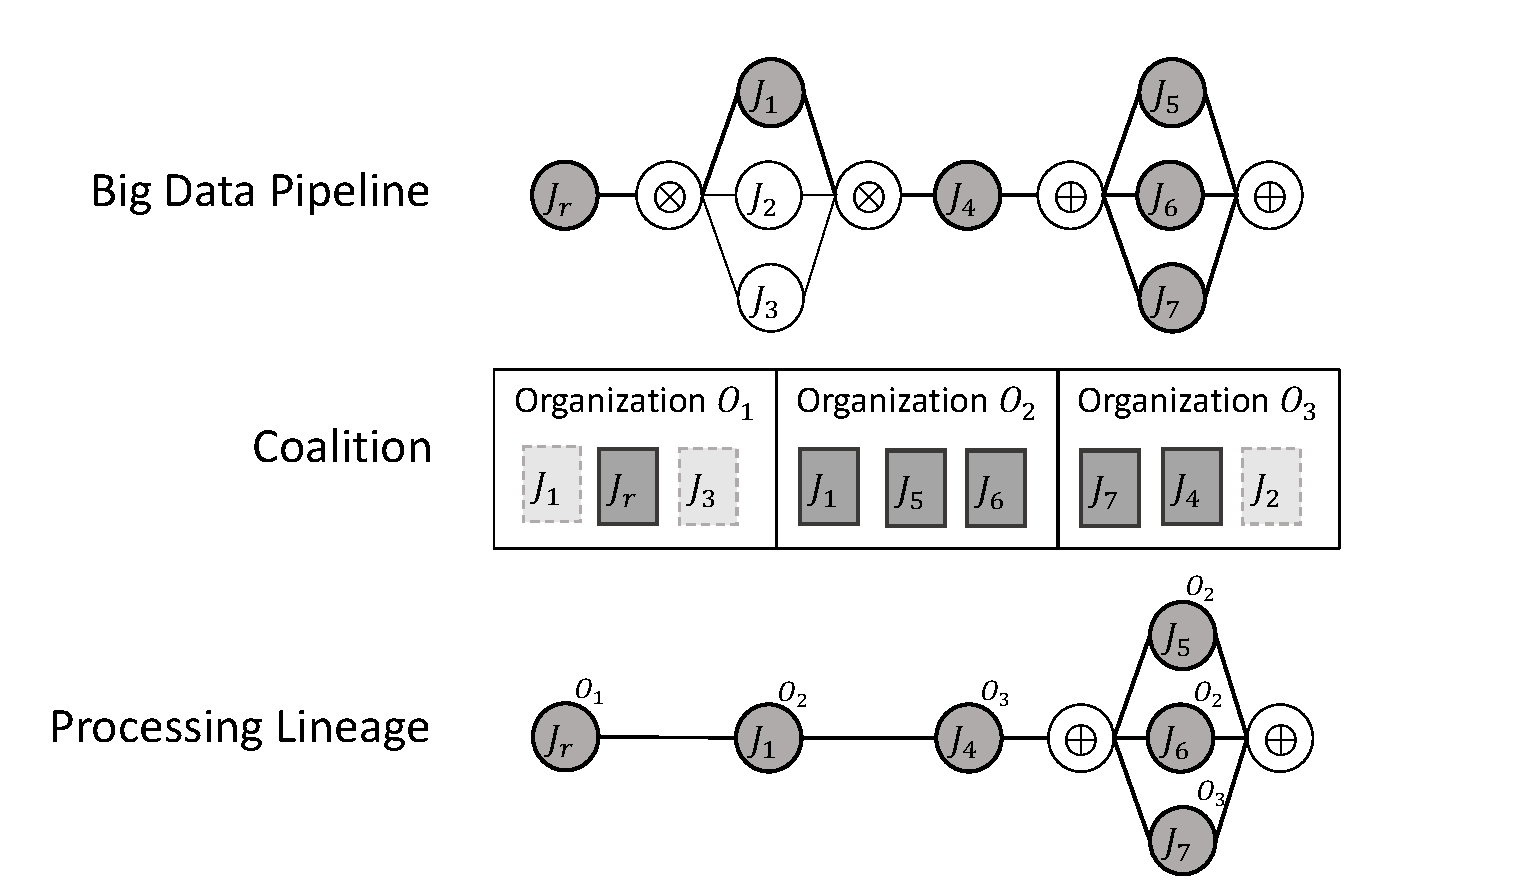
\includegraphics[width=0.98\columnwidth]{generaleFig1.pdf}
  \caption{Big Data Analytics pipeline graphs with a coalition of organization for a given processing lineage.}\label{fig:BDpipeline}
\end{figure}

Figure~\ref{fig:BDpipeline} shows an overview of our system model.

%Solid arrows present the typical batch or analytics model generation flows. Dashed arrows present typical streaming or prediction flows. \CH{togliere dalla figura la linea che separa le due procedure e le scritte ingestion procedure e analytics procedure?}
%The coalition creation is driven by missions including emergency and disaster management, humanitarian operations, or simply interdependent organizations.
%\CH{Qui ho introdotto solo il termine coalition, va spiegato anche il termine federation?}
\subsection{Reference Scenario}
Our reference scenario is a service-based environment where services are composed according to a pipeline template.
Our case study is grounded in the analysis of a dataset comprising individuals held in Department of Correction facilities in the state of Connecticut while awaiting trial.
The dataset\footnote{https://data.ct.gov/Public-Safety/Accused-Pre-Trial-Inmates-in-Correctional-Faciliti/b674-jy6w}, exhibits a straightforward row-and-column structure.
Each row represents an inmate, and the columns include the following attributes: date of download, a unique identifier, last entry date, "race," gender, age of the individual, the bound value, offense, entry facility, and detainer.
To serve the objectives of our study, we have extended this dataset by introducing randomly generated first and last names.

Within the context of our case study, we envision the establishment of a service pipeline designed as follows:
The end user, a member of the Connecticut Department of Correction (DOC),
seeks to perform an analysis on the dataset to compare admission trends in Connecticut prisons with those in other states.
The user's preferences align with a predefined template that orchestrates the following sequence of operations:
i) Anonymization of the dataset.
ii) Expansion of the dataset, integrating data from the states of New York and New Hampshire.
iii) Transformation of the dataset to derive state-specific data aggregations, including statistical measures like averages, medians, and clustering-based statistics.
iv) Storage of the resultant data in reference states. Specifically, one copy remains in Connecticut (where sensitive information in the source dataset is not protected), while two additional copies are distributed to New York and New Hampshire (with sensitive information from the source dataset being safeguarded).

It is important to note that the template mandates that the entire service is executed within a single country, and any instance where the data must traverse beyond the boundaries of Connecticut, rigorous data protection measures are implemented.
A visual representation of the template is presented in Figure \ref{fig:service_composition_example}.

At each service you can see examples of the use of the f and lambda functions.
In the first step That of anonymization the service f is empty since the service does not apply any transformation.
The anonymization is in fact borne by the policy via the \myLambda function.
In the second step of expansion the function is adoptive in that it extends the dataset by merging it with other sources, the policy instead only enforces execution on Connecticut territory.
In the third step the transformation one the Function is transformational in that it aggregates the data to extract statistics from it the policy is the same as in step 2, finally in the last step the transformation F is empty in that the service only stores the dataset.
The policy instead performs an anonymization just on the geolocation


\begin{figure}
  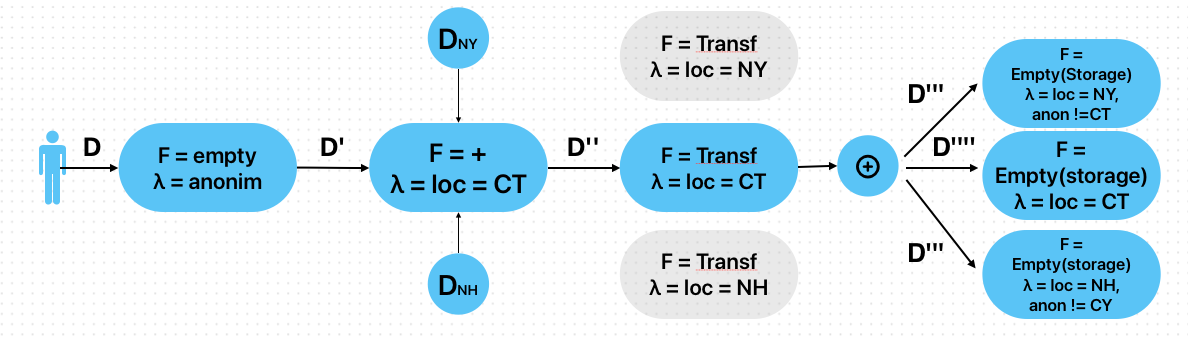
\includegraphics[width=0.98\columnwidth]{service_composition_example}
  \caption{Service composition example.}\label{fig:service_composition_example}

\end{figure}
\section{Policy}

\subsection{Annotations}
\subsection{Transformation}
\subsection{Policy}

\subsubsection{Policy Decision/Policy Matching}
\subsubsection{Policy Enforcement}
\subsubsection{Policy Evaluation}